% Inverse loop fixture: a.tex with wording and inline styles changed.
\documentclass{beamer}
\setbeamertemplate{navigation symbols}{}
\graphicspath{{img/}}
\title{Inverse Conversion}
\author{Test Author}
\date{17 September 2026}

\begin{document}

\begin{frame}[label=title]
  \titlepage
\end{frame}

\begin{frame}[label=motivation]{Why convert back}
  \begin{itemize}
    \item Decks are edited after they are converted
    \item The source should follow the deck
      \begin{itemize}
        \item without losing \textbf{semantic} markup
        \item and without rewriting untouched frames
      \end{itemize}
    \item Every edit is checked by compiling again
  \end{itemize}
\end{frame}

\begin{frame}[label=method]{Method}
  We compile the candidate, \textbf{classify} the PDF and compare it with the
  target deck, \textcolor{red}{word by word} and box by box.

  Residuals turn into source edits until nothing is left.
\end{frame}

\begin{frame}[label=results]{Results so far}
  \begin{enumerate}
    \item Text edits converge in one round
    \item Moves need a second round
    \item Lists keep their items
  \end{enumerate}
  \note{Mention the iteration counts.}
\end{frame}

\begin{frame}[label=picture]{A picture}
  \centering
  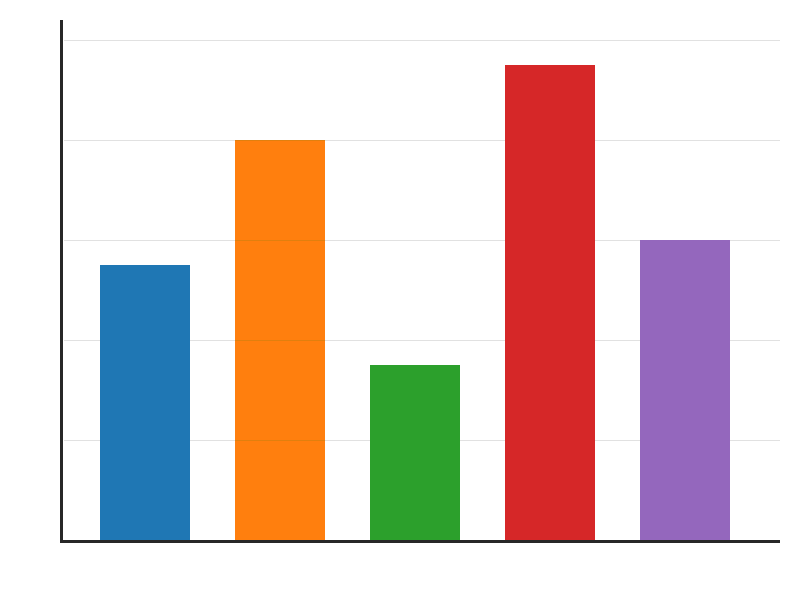
\includegraphics[width=0.5\textwidth]{plot.png}

  A chart of five groups.
\end{frame}

\end{document}
